%-*-latex-*-
\sectionthree{Tree}
\begin{python0}
from solutions import *; clear()
\end{python0}

A tree is just a connected graph without cycles.
In this case, I'm talking about a tree as an undirected
graph.
You have to be careful, sometimes, a tree can also 
refer to a tree as a directed graph and acyclic.

Sometimes a special node is selected.
In this case, such a tree is sometimes called a rooted tree
(or a tree with a root).

Here's a tree (directed version):

%-*-latex-*-
{\footnotesize \begin{Verbatim}[frame=single,fontsize=\small]
[student@localhost discrete-probability] python tossfaircoin1.py
experiment 0 ... outcome: HEAD
experiment 1 ... outcome: TAIL
experiment 2 ... outcome: HEAD
experiment 3 ... outcome: TAIL
experiment 4 ... outcome: HEAD
experiment 5 ... outcome: TAIL
experiment 6 ... outcome: TAIL
experiment 7 ... outcome: TAIL
experiment 8 ... outcome: TAIL
experiment 9 ... outcome: TAIL
experiment 10 ... outcome: TAIL
experiment 11 ... outcome: HEAD
experiment 12 ... outcome: HEAD
experiment 13 ... outcome: TAIL
experiment 14 ... outcome: HEAD
experiment 15 ... outcome: HEAD
experiment 16 ... outcome: HEAD
experiment 17 ... outcome: TAIL
experiment 18 ... outcome: TAIL
experiment 19 ... outcome: HEAD
\end{Verbatim}
}


\begin{myenum}

  \li
  $a$ is the \defone{root} of the tree.

  \li
  $a$ has 3 \defone{children}, i.e., $b,c,d$; 
  $a$ has a
  \sidebarskip{8pt}
  \defone{branching factor} 
  of 3.
  Sometimes, it's convenient to number the children.
  I'll call $b$ child $0$ of $a$; $d$ is child $2$ of $a$.

  \li
  $a$ is the \defone{parent} of $b$.

  \li
  $k$,$l$,$f$,$g$,$m$,$i$,$j$ are called
  \sidebarskip{-2pt}
  \defone{leaves}
  or
  \sidebarskip{12pt}\defone{non-internal} nodes because
  they don't have children.

  \li
  $a,b,c,d,e,h$ are called
  \sidebarskip{-2pt}
  \defone{non-leaf} nodes or 
  \sidebarskip{12pt}\defone{internal} nodes because 
  each have at least one child.

  \li
  $b$ has a \defone{depth} of $1$, i.e., 
  the length of the path from the root to $b$
  is 1. I will also say that $b$ is at level $1$.
  A root (see $a$ above) has depth 0.

  \li
  $b$ has a \defone{height} of $2$, i.e., 
  the length of the longest path from 
  $b$ to a leaf is 2.
  A leaf (see $k$ above) has height 0.

  \li
  The \defone{height} of a tree is the height of the root of the tree.
  The above tree has a height of 3.
  The height of an empty tree is -1.

  \li
  The root is at level 0. $b,c,d$ are at level 1.
  $e,f,g,h,i,j$ are at level 2. $k,l,m$ are at level 3.
  
  \li
  Two nodes $u$ and $v$ are \defone{siblings} if they have
  the same parent.
  For instance $b,c,d$ are siblings.
  
  \li
  $u$ has \defone{descendent} $v$ if there is a sequence of nodes 
  $u = v_0$, $v_1$, ..., $v_n = v$ where $v_i$ is the parent of $v_{i+1}$.
  $v$ is the \defone{ancestor} of $u$ if $u$ is a descendent of $v$.
  For instance in the above tree $b$ is an ancestor of $i$ and
  $i$ is a descendent of $l$.

\end{myenum}
Note that the above tree is a directed graph.
The following is also a tree (as in an \textit{undirected} tree).

\begin{center}
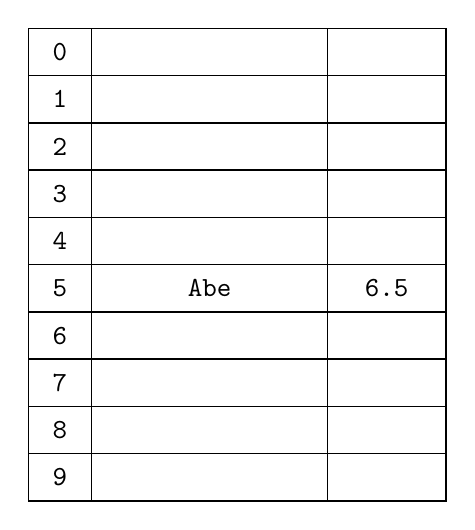
\begin{tikzpicture}

\draw (1.4, 0.7)
  node[draw, line width=0.02cm, , color=black,
       rounded corners=0cm, inner sep=0cm] {

\begin{minipage}[t][0.6cm]{0.8cm}
\mbox{}

\end{minipage}

};\draw (1.4, 0.7) node[color=black] {{\texttt{0}}};
\draw (3.3, 0.7)
  node[draw, line width=0.02cm, , color=black,
       rounded corners=0cm, inner sep=0cm] {

\begin{minipage}[t][0.6cm]{3.0cm}
\mbox{}

\end{minipage}

};\draw (3.3, 0.7) node[color=black] {{\texttt{}}};
\draw (5.55, 0.7)
  node[draw, line width=0.02cm, , color=black,
       rounded corners=0cm, inner sep=0cm] {

\begin{minipage}[t][0.6cm]{1.5cm}
\mbox{}

\end{minipage}

};\draw (5.55, 0.7) node[color=black] {{\texttt{}}};
\draw (1.4, 0.09999999999999987)
  node[draw, line width=0.02cm, , color=black,
       rounded corners=0cm, inner sep=0cm] {

\begin{minipage}[t][0.6cm]{0.8cm}
\mbox{}

\end{minipage}

};\draw (1.4, 0.09999999999999987) node[color=black] {{\texttt{1}}};
\draw (3.3, 0.09999999999999987)
  node[draw, line width=0.02cm, , color=black,
       rounded corners=0cm, inner sep=0cm] {

\begin{minipage}[t][0.6cm]{3.0cm}
\mbox{}

\end{minipage}

};\draw (3.3, 0.09999999999999987) node[color=black] {{\texttt{}}};
\draw (5.55, 0.09999999999999987)
  node[draw, line width=0.02cm, , color=black,
       rounded corners=0cm, inner sep=0cm] {

\begin{minipage}[t][0.6cm]{1.5cm}
\mbox{}

\end{minipage}

};\draw (5.55, 0.09999999999999987) node[color=black] {{\texttt{}}};
\draw (1.4, -0.5000000000000002)
  node[draw, line width=0.02cm, , color=black,
       rounded corners=0cm, inner sep=0cm] {

\begin{minipage}[t][0.6cm]{0.8cm}
\mbox{}

\end{minipage}

};\draw (1.4, -0.5000000000000002) node[color=black] {{\texttt{2}}};
\draw (3.3, -0.5000000000000002)
  node[draw, line width=0.02cm, , color=black,
       rounded corners=0cm, inner sep=0cm] {

\begin{minipage}[t][0.6cm]{3.0cm}
\mbox{}

\end{minipage}

};\draw (3.3, -0.5000000000000002) node[color=black] {{\texttt{}}};
\draw (5.55, -0.5000000000000002)
  node[draw, line width=0.02cm, , color=black,
       rounded corners=0cm, inner sep=0cm] {

\begin{minipage}[t][0.6cm]{1.5cm}
\mbox{}

\end{minipage}

};\draw (5.55, -0.5000000000000002) node[color=black] {{\texttt{}}};
\draw (1.4, -1.1000000000000003)
  node[draw, line width=0.02cm, , color=black,
       rounded corners=0cm, inner sep=0cm] {

\begin{minipage}[t][0.6cm]{0.8cm}
\mbox{}

\end{minipage}

};\draw (1.4, -1.1000000000000003) node[color=black] {{\texttt{3}}};
\draw (3.3, -1.1000000000000003)
  node[draw, line width=0.02cm, , color=black,
       rounded corners=0cm, inner sep=0cm] {

\begin{minipage}[t][0.6cm]{3.0cm}
\mbox{}

\end{minipage}

};\draw (3.3, -1.1000000000000003) node[color=black] {{\texttt{}}};
\draw (5.55, -1.1000000000000003)
  node[draw, line width=0.02cm, , color=black,
       rounded corners=0cm, inner sep=0cm] {

\begin{minipage}[t][0.6cm]{1.5cm}
\mbox{}

\end{minipage}

};\draw (5.55, -1.1000000000000003) node[color=black] {{\texttt{}}};
\draw (1.4, -1.7000000000000002)
  node[draw, line width=0.02cm, , color=black,
       rounded corners=0cm, inner sep=0cm] {

\begin{minipage}[t][0.6cm]{0.8cm}
\mbox{}

\end{minipage}

};\draw (1.4, -1.7000000000000002) node[color=black] {{\texttt{4}}};
\draw (3.3, -1.7000000000000002)
  node[draw, line width=0.02cm, , color=black,
       rounded corners=0cm, inner sep=0cm] {

\begin{minipage}[t][0.6cm]{3.0cm}
\mbox{}

\end{minipage}

};\draw (3.3, -1.7000000000000002) node[color=black] {{\texttt{}}};
\draw (5.55, -1.7000000000000002)
  node[draw, line width=0.02cm, , color=black,
       rounded corners=0cm, inner sep=0cm] {

\begin{minipage}[t][0.6cm]{1.5cm}
\mbox{}

\end{minipage}

};\draw (5.55, -1.7000000000000002) node[color=black] {{\texttt{}}};
\draw (1.4, -2.3000000000000003)
  node[draw, line width=0.02cm, , color=black,
       rounded corners=0cm, inner sep=0cm] {

\begin{minipage}[t][0.6cm]{0.8cm}
\mbox{}

\end{minipage}

};\draw (1.4, -2.3000000000000003) node[color=black] {{\texttt{5}}};
\draw (3.3, -2.3000000000000003)
  node[draw, line width=0.02cm, , color=black,
       rounded corners=0cm, inner sep=0cm] {

\begin{minipage}[t][0.6cm]{3.0cm}
\mbox{}

\end{minipage}

};\draw (3.3, -2.3000000000000003) node[color=black] {{\texttt{Abe}}};
\draw (5.55, -2.3000000000000003)
  node[draw, line width=0.02cm, , color=black,
       rounded corners=0cm, inner sep=0cm] {

\begin{minipage}[t][0.6cm]{1.5cm}
\mbox{}

\end{minipage}

};\draw (5.55, -2.3000000000000003) node[color=black] {{\texttt{6.5}}};
\draw (1.4, -2.9000000000000004)
  node[draw, line width=0.02cm, , color=black,
       rounded corners=0cm, inner sep=0cm] {

\begin{minipage}[t][0.6cm]{0.8cm}
\mbox{}

\end{minipage}

};\draw (1.4, -2.9000000000000004) node[color=black] {{\texttt{6}}};
\draw (3.3, -2.9000000000000004)
  node[draw, line width=0.02cm, , color=black,
       rounded corners=0cm, inner sep=0cm] {

\begin{minipage}[t][0.6cm]{3.0cm}
\mbox{}

\end{minipage}

};\draw (3.3, -2.9000000000000004) node[color=black] {{\texttt{}}};
\draw (5.55, -2.9000000000000004)
  node[draw, line width=0.02cm, , color=black,
       rounded corners=0cm, inner sep=0cm] {

\begin{minipage}[t][0.6cm]{1.5cm}
\mbox{}

\end{minipage}

};\draw (5.55, -2.9000000000000004) node[color=black] {{\texttt{}}};
\draw (1.4, -3.500000000000001)
  node[draw, line width=0.02cm, , color=black,
       rounded corners=0cm, inner sep=0cm] {

\begin{minipage}[t][0.6cm]{0.8cm}
\mbox{}

\end{minipage}

};\draw (1.4, -3.500000000000001) node[color=black] {{\texttt{7}}};
\draw (3.3, -3.500000000000001)
  node[draw, line width=0.02cm, , color=black,
       rounded corners=0cm, inner sep=0cm] {

\begin{minipage}[t][0.6cm]{3.0cm}
\mbox{}

\end{minipage}

};\draw (3.3, -3.500000000000001) node[color=black] {{\texttt{}}};
\draw (5.55, -3.500000000000001)
  node[draw, line width=0.02cm, , color=black,
       rounded corners=0cm, inner sep=0cm] {

\begin{minipage}[t][0.6cm]{1.5cm}
\mbox{}

\end{minipage}

};\draw (5.55, -3.500000000000001) node[color=black] {{\texttt{}}};
\draw (1.4, -4.1000000000000005)
  node[draw, line width=0.02cm, , color=black,
       rounded corners=0cm, inner sep=0cm] {

\begin{minipage}[t][0.6cm]{0.8cm}
\mbox{}

\end{minipage}

};\draw (1.4, -4.1000000000000005) node[color=black] {{\texttt{8}}};
\draw (3.3, -4.1000000000000005)
  node[draw, line width=0.02cm, , color=black,
       rounded corners=0cm, inner sep=0cm] {

\begin{minipage}[t][0.6cm]{3.0cm}
\mbox{}

\end{minipage}

};\draw (3.3, -4.1000000000000005) node[color=black] {{\texttt{}}};
\draw (5.55, -4.1000000000000005)
  node[draw, line width=0.02cm, , color=black,
       rounded corners=0cm, inner sep=0cm] {

\begin{minipage}[t][0.6cm]{1.5cm}
\mbox{}

\end{minipage}

};\draw (5.55, -4.1000000000000005) node[color=black] {{\texttt{}}};
\draw (1.4, -4.7)
  node[draw, line width=0.02cm, , color=black,
       rounded corners=0cm, inner sep=0cm] {

\begin{minipage}[t][0.6cm]{0.8cm}
\mbox{}

\end{minipage}

};\draw (1.4, -4.7) node[color=black] {{\texttt{9}}};
\draw (3.3, -4.7)
  node[draw, line width=0.02cm, , color=black,
       rounded corners=0cm, inner sep=0cm] {

\begin{minipage}[t][0.6cm]{3.0cm}
\mbox{}

\end{minipage}

};\draw (3.3, -4.7) node[color=black] {{\texttt{}}};
\draw (5.55, -4.7)
  node[draw, line width=0.02cm, , color=black,
       rounded corners=0cm, inner sep=0cm] {

\begin{minipage}[t][0.6cm]{1.5cm}
\mbox{}

\end{minipage}

};\draw (5.55, -4.7) node[color=black] {{\texttt{}}};
\end{tikzpicture}

\end{center}



In the case of implementation, you can think of the directed version
as having pointers from a parent to the children.
In the case of the undirected version, you can think of
each edge as allowing you to go both up and down -- 
nodes having pointers going to their children or parent.
Of course exceptions being that roots have no parents and leaves have no
children.

For each node of a tree $T$, if you consider all the descendents of the node, 
you have a tree. This is called a \defone{subtree} of $T$.
For instance

\begin{center}
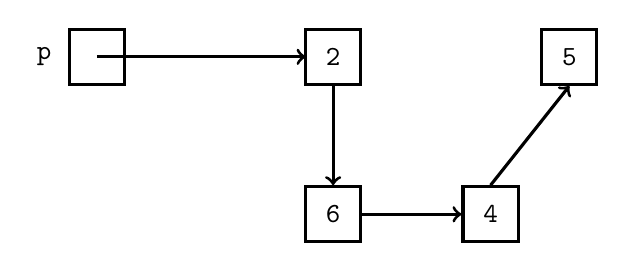
\begin{tikzpicture}

\draw (0.35, 0.35)
  node[draw, line width=0.04cm, , color=black,
       rounded corners=0cm, inner sep=0cm] {

\begin{minipage}[t][0.7cm]{0.7cm}
\mbox{}

\end{minipage}

};\draw (0.35, 0.35) node[color=black] {{\texttt{2}}};
\draw (0.35, -1.65)
  node[draw, line width=0.04cm, , color=black,
       rounded corners=0cm, inner sep=0cm] {

\begin{minipage}[t][0.7cm]{0.7cm}
\mbox{}

\end{minipage}

};\draw (0.35, -1.65) node[color=black] {{\texttt{6}}};
\draw (2.35, -1.65)
  node[draw, line width=0.04cm, , color=black,
       rounded corners=0cm, inner sep=0cm] {

\begin{minipage}[t][0.7cm]{0.7cm}
\mbox{}

\end{minipage}

};\draw (2.35, -1.65) node[color=black] {{\texttt{4}}};
\draw (3.35, 0.35)
  node[draw, line width=0.04cm, , color=black,
       rounded corners=0cm, inner sep=0cm] {

\begin{minipage}[t][0.7cm]{0.7cm}
\mbox{}

\end{minipage}

};\draw (3.35, 0.35) node[color=black] {{\texttt{5}}};\draw[line width=0.04cm,black,->] (0.35,-0.02) to  (0.35,-1.28);
\draw[line width=0.04cm,black,->] (0.72,-1.65) to  (1.98,-1.65);
\draw[line width=0.04cm,black,->] (2.35,-1.28) to  (3.35,-0.02);

\draw (-2.65, 0.35)
  node[draw, line width=0.04cm, , color=black,
       rounded corners=0cm, inner sep=0cm] {

\begin{minipage}[t][0.7cm]{0.7cm}
\mbox{}

\end{minipage}

};\draw (-2.65, 0.35) node[color=black] {{\texttt{}}};\draw[line width=0.04cm,black,->] (-2.65,0.35) to  (0,0.35);

\draw (-3.32, 0.35)
  node[draw, line width=0.04cm, , color=white,
       rounded corners=0cm, inner sep=0cm] {

\begin{minipage}[t][0.1cm]{0.1cm}
\mbox{}

\end{minipage}

};\draw (-3.32, 0.35) node[color=black] {{\texttt{p}}};
\end{tikzpicture}

\end{center}



is a subtree of 

\begin{center}
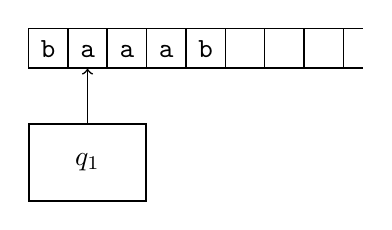
\begin{tikzpicture}

\draw (0.25, 0.25)
  node[draw, line width=0.02cm, , color=black,
       rounded corners=0cm, inner sep=0cm] {

\begin{minipage}[t][0.5cm]{0.5cm}
\mbox{}

\end{minipage}

};\draw (0.25, 0.25) node[color=black] {{\vphantom{baaab\SPACE\SPACE\SPACE}\texttt{b}}};
\draw (0.75, 0.25)
  node[draw, line width=0.02cm, , color=black,
       rounded corners=0cm, inner sep=0cm] {

\begin{minipage}[t][0.5cm]{0.5cm}
\mbox{}

\end{minipage}

};\draw (0.75, 0.25) node[color=black] {{\vphantom{baaab\SPACE\SPACE\SPACE}\texttt{a}}};
\draw (1.25, 0.25)
  node[draw, line width=0.02cm, , color=black,
       rounded corners=0cm, inner sep=0cm] {

\begin{minipage}[t][0.5cm]{0.5cm}
\mbox{}

\end{minipage}

};\draw (1.25, 0.25) node[color=black] {{\vphantom{baaab\SPACE\SPACE\SPACE}\texttt{a}}};
\draw (1.75, 0.25)
  node[draw, line width=0.02cm, , color=black,
       rounded corners=0cm, inner sep=0cm] {

\begin{minipage}[t][0.5cm]{0.5cm}
\mbox{}

\end{minipage}

};\draw (1.75, 0.25) node[color=black] {{\vphantom{baaab\SPACE\SPACE\SPACE}\texttt{a}}};
\draw (2.25, 0.25)
  node[draw, line width=0.02cm, , color=black,
       rounded corners=0cm, inner sep=0cm] {

\begin{minipage}[t][0.5cm]{0.5cm}
\mbox{}

\end{minipage}

};\draw (2.25, 0.25) node[color=black] {{\vphantom{baaab\SPACE\SPACE\SPACE}\texttt{b}}};
\draw (2.75, 0.25)
  node[draw, line width=0.02cm, , color=black,
       rounded corners=0cm, inner sep=0cm] {

\begin{minipage}[t][0.5cm]{0.5cm}
\mbox{}

\end{minipage}

};\draw (2.75, 0.25) node[color=black] {{\vphantom{baaab\SPACE\SPACE\SPACE}\texttt{\SPACE}}};
\draw (3.25, 0.25)
  node[draw, line width=0.02cm, , color=black,
       rounded corners=0cm, inner sep=0cm] {

\begin{minipage}[t][0.5cm]{0.5cm}
\mbox{}

\end{minipage}

};\draw (3.25, 0.25) node[color=black] {{\vphantom{baaab\SPACE\SPACE\SPACE}\texttt{\SPACE}}};
\draw (3.75, 0.25)
  node[draw, line width=0.02cm, , color=black,
       rounded corners=0cm, inner sep=0cm] {

\begin{minipage}[t][0.5cm]{0.5cm}
\mbox{}

\end{minipage}

};\draw (3.75, 0.25) node[color=black] {{\vphantom{baaab\SPACE\SPACE\SPACE}\texttt{\SPACE}}};\draw[line width=0.02cm,black] (4.0,0.5) to  (4.25,0.5);
\draw[line width=0.02cm,black] (4.0,0.0) to  (4.25,0.0);

\draw (0.75, -1.2)
  node[draw, line width=0.02cm, , color=black,
       rounded corners=0cm, inner sep=0cm] {

\begin{minipage}[t][0.98cm]{1.48cm}
\mbox{}

\end{minipage}

};\draw (0.75, -1.2) node[color=black] {$q_1$};\draw[line width=0.02cm,black,->] (0.75,-0.7) to  (0.75,-0.47) to  (0.75,-0.47) to  (0.75,-0.01);
\end{tikzpicture}

\end{center}



I will say that this is the subtree at $b$.

In the case of a node with two child, 
there are two subtrees, the subtree on the left is called the 
\defone{left subtree} and the one on the right is called the 
\defone{right subtree}.
(Duh.)
Look at the subtree at $b$:

\begin{center}
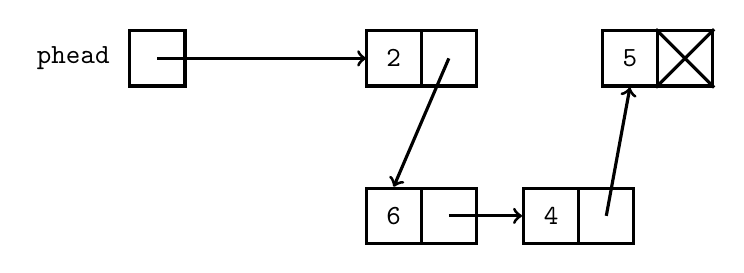
\begin{tikzpicture}

\draw (0.35, 0.35)
  node[draw, line width=0.04cm, , color=black,
       rounded corners=0cm, inner sep=0cm] {

\begin{minipage}[t][0.7cm]{0.7cm}
\mbox{}

\end{minipage}

};\draw (0.35, 0.35) node[color=black] {{\texttt{2}}};
\draw (1.0499999999999998, 0.35)
  node[draw, line width=0.04cm, , color=black,
       rounded corners=0cm, inner sep=0cm] {

\begin{minipage}[t][0.7cm]{0.7cm}
\mbox{}

\end{minipage}

};\draw (1.0499999999999998, 0.35) node[color=black] {{\texttt{}}};
\draw (0.35, -1.65)
  node[draw, line width=0.04cm, , color=black,
       rounded corners=0cm, inner sep=0cm] {

\begin{minipage}[t][0.7cm]{0.7cm}
\mbox{}

\end{minipage}

};\draw (0.35, -1.65) node[color=black] {{\texttt{6}}};
\draw (1.0499999999999998, -1.65)
  node[draw, line width=0.04cm, , color=black,
       rounded corners=0cm, inner sep=0cm] {

\begin{minipage}[t][0.7cm]{0.7cm}
\mbox{}

\end{minipage}

};\draw (1.0499999999999998, -1.65) node[color=black] {{\texttt{}}};
\draw (2.35, -1.65)
  node[draw, line width=0.04cm, , color=black,
       rounded corners=0cm, inner sep=0cm] {

\begin{minipage}[t][0.7cm]{0.7cm}
\mbox{}

\end{minipage}

};\draw (2.35, -1.65) node[color=black] {{\texttt{4}}};
\draw (3.0500000000000003, -1.65)
  node[draw, line width=0.04cm, , color=black,
       rounded corners=0cm, inner sep=0cm] {

\begin{minipage}[t][0.7cm]{0.7cm}
\mbox{}

\end{minipage}

};\draw (3.0500000000000003, -1.65) node[color=black] {{\texttt{}}};
\draw (3.35, 0.35)
  node[draw, line width=0.04cm, , color=black,
       rounded corners=0cm, inner sep=0cm] {

\begin{minipage}[t][0.7cm]{0.7cm}
\mbox{}

\end{minipage}

};\draw (3.35, 0.35) node[color=black] {{\texttt{5}}};
\draw (4.05, 0.35)
  node[draw, line width=0.04cm, , color=black,
       rounded corners=0cm, inner sep=0cm] {

\begin{minipage}[t][0.7cm]{0.7cm}
\mbox{}

\end{minipage}

};\draw (4.05, 0.35) node[color=black] {{\texttt{}}};\draw[line width=0.04cm,black,->] (1.05,0.35) to  (0.35,-1.28);
\draw[line width=0.04cm,black,->] (1.05,-1.65) to  (1.98,-1.65);
\draw[line width=0.04cm,black,->] (3.05,-1.65) to  (3.35,-0.02);
\draw[line width=0.04cm,black] (3.68,0.72) to  (4.42,-0.02);
\draw[line width=0.04cm,black] (4.42,0.72) to  (3.68,-0.02);

\draw (-2.65, 0.35)
  node[draw, line width=0.04cm, , color=black,
       rounded corners=0cm, inner sep=0cm] {

\begin{minipage}[t][0.7cm]{0.7cm}
\mbox{}

\end{minipage}

};\draw (-2.65, 0.35) node[color=black] {{\texttt{}}};\draw[line width=0.04cm,black,->] (-2.65,0.35) to  (0,0.35);

\draw (-3.7199999999999998, 0.35)
  node[draw, line width=0.04cm, , color=white,
       rounded corners=0cm, inner sep=0cm] {

\begin{minipage}[t][0.1cm]{0.1cm}
\mbox{}

\end{minipage}

};\draw (-3.7199999999999998, 0.35) node[color=black] {{\texttt{phead}}};
\end{tikzpicture}

\end{center}



The nodes $e,k,l$ form the left subtree of $b$
and the single node $f$ form the right subtree of $b$.


A tree is said to be \defone{$k$--ary} if every node has at most $k$ children;
that's the same as saying that every node has a maximum branching factor of
$k$.
In particular, a \defone{binary} tree is a tree with at most 2 children.

%-*-latex-*-

\begin{ex} 
  \label{ex:prob-00}
  \tinysidebar{\debug{exercises/{disc-prob-28/question.tex}}}

  \solutionlink{sol:prob-00}
  \qed
\end{ex} 
\begin{python0}
from solutions import *
add(label="ex:prob-00",
    srcfilename='exercises/discrete-probability/prob-00/answer.tex') 
\end{python0}


We include the empty graph as a tree, except of course such trees
don't have roots.
Consider a $k$--ary tree $T$.
\begin{myenum}

\li $T$ is \defone{full} if every node has exactly $k$ children, except for 
the leaves, i.e., if every node has
either $k$ or $0$ children.
Here's a full binary tree:

\begin{center}
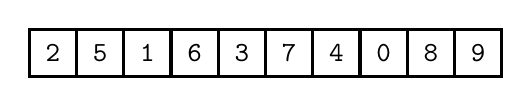
\begin{tikzpicture}

\draw (0.3, -0.3)
  node[draw, line width=0.04cm, , color=black,
       rounded corners=0cm, inner sep=0cm] {

\begin{minipage}[t][0.6cm]{0.6cm}
\mbox{}

\end{minipage}

};\draw (0.3, -0.3) node[color=black] {{\texttt{2}}};
\draw (0.8999999999999999, -0.3)
  node[draw, line width=0.04cm, , color=black,
       rounded corners=0cm, inner sep=0cm] {

\begin{minipage}[t][0.6cm]{0.6cm}
\mbox{}

\end{minipage}

};\draw (0.8999999999999999, -0.3) node[color=black] {{\texttt{5}}};
\draw (1.5, -0.3)
  node[draw, line width=0.04cm, , color=black,
       rounded corners=0cm, inner sep=0cm] {

\begin{minipage}[t][0.6cm]{0.6cm}
\mbox{}

\end{minipage}

};\draw (1.5, -0.3) node[color=black] {{\texttt{1}}};
\draw (2.0999999999999996, -0.3)
  node[draw, line width=0.04cm, , color=black,
       rounded corners=0cm, inner sep=0cm] {

\begin{minipage}[t][0.6cm]{0.6cm}
\mbox{}

\end{minipage}

};\draw (2.0999999999999996, -0.3) node[color=black] {{\texttt{6}}};
\draw (2.7, -0.3)
  node[draw, line width=0.04cm, , color=black,
       rounded corners=0cm, inner sep=0cm] {

\begin{minipage}[t][0.6cm]{0.6cm}
\mbox{}

\end{minipage}

};\draw (2.7, -0.3) node[color=black] {{\texttt{3}}};
\draw (3.3, -0.3)
  node[draw, line width=0.04cm, , color=black,
       rounded corners=0cm, inner sep=0cm] {

\begin{minipage}[t][0.6cm]{0.6cm}
\mbox{}

\end{minipage}

};\draw (3.3, -0.3) node[color=black] {{\texttt{7}}};
\draw (3.9, -0.3)
  node[draw, line width=0.04cm, , color=black,
       rounded corners=0cm, inner sep=0cm] {

\begin{minipage}[t][0.6cm]{0.6cm}
\mbox{}

\end{minipage}

};\draw (3.9, -0.3) node[color=black] {{\texttt{4}}};
\draw (4.5, -0.3)
  node[draw, line width=0.04cm, , color=black,
       rounded corners=0cm, inner sep=0cm] {

\begin{minipage}[t][0.6cm]{0.6cm}
\mbox{}

\end{minipage}

};\draw (4.5, -0.3) node[color=black] {{\texttt{0}}};
\draw (5.1, -0.3)
  node[draw, line width=0.04cm, , color=black,
       rounded corners=0cm, inner sep=0cm] {

\begin{minipage}[t][0.6cm]{0.6cm}
\mbox{}

\end{minipage}

};\draw (5.1, -0.3) node[color=black] {{\texttt{8}}};
\draw (5.699999999999999, -0.3)
  node[draw, line width=0.04cm, , color=black,
       rounded corners=0cm, inner sep=0cm] {

\begin{minipage}[t][0.6cm]{0.6cm}
\mbox{}

\end{minipage}

};\draw (5.699999999999999, -0.3) node[color=black] {{\texttt{9}}};
\end{tikzpicture}

\end{center}



Here's another:

\begin{center}
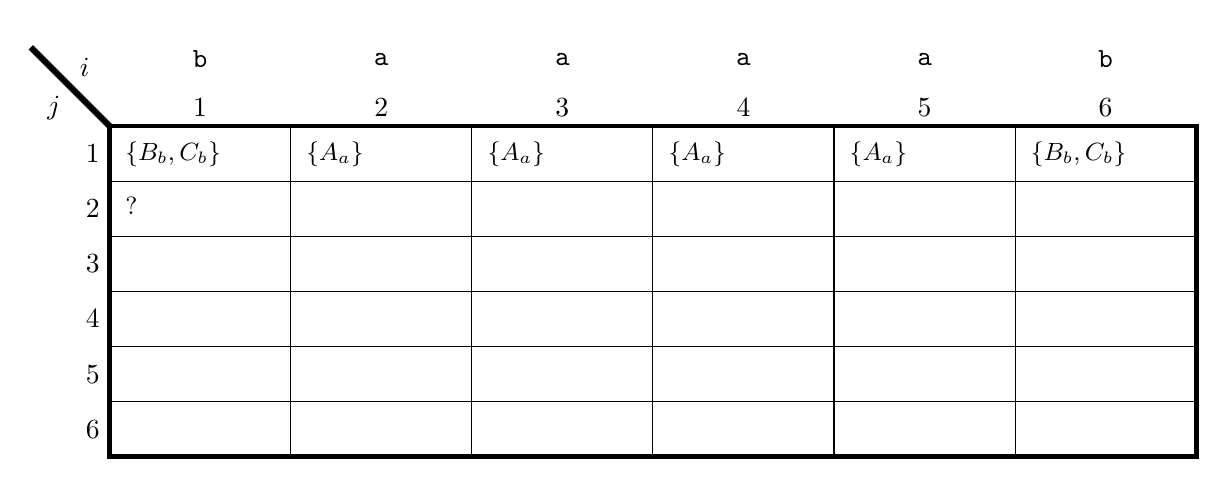
\begin{tikzpicture}

\draw (1.15, -0.35)
  node[draw, , , color=black,
       rounded corners=0cm, inner sep=0.2cm] {

\begin{minipage}[t][0.3cm]{1.9cm}
\mbox{}

\end{minipage}

};
\draw (1.15, -0.35) node[color=black,
 inner sep=0.2cm] {
 
\begin{minipage}[t][0.3cm]{1.9cm}
{\small $\{B_b,C_b\}$}
\end{minipage}

};
\draw (3.4499999999999997, -0.35)
  node[draw, , , color=black,
       rounded corners=0cm, inner sep=0.2cm] {

\begin{minipage}[t][0.3cm]{1.9cm}
\mbox{}

\end{minipage}

};
\draw (3.4499999999999997, -0.35) node[color=black,
 inner sep=0.2cm] {
 
\begin{minipage}[t][0.3cm]{1.9cm}
{\small $\{A_a\}$}
\end{minipage}

};
\draw (5.75, -0.35)
  node[draw, , , color=black,
       rounded corners=0cm, inner sep=0.2cm] {

\begin{minipage}[t][0.3cm]{1.9cm}
\mbox{}

\end{minipage}

};
\draw (5.75, -0.35) node[color=black,
 inner sep=0.2cm] {
 
\begin{minipage}[t][0.3cm]{1.9cm}
{\small $\{A_a\}$}
\end{minipage}

};
\draw (8.049999999999999, -0.35)
  node[draw, , , color=black,
       rounded corners=0cm, inner sep=0.2cm] {

\begin{minipage}[t][0.3cm]{1.9cm}
\mbox{}

\end{minipage}

};
\draw (8.049999999999999, -0.35) node[color=black,
 inner sep=0.2cm] {
 
\begin{minipage}[t][0.3cm]{1.9cm}
{\small $\{A_a\}$}
\end{minipage}

};
\draw (10.35, -0.35)
  node[draw, , , color=black,
       rounded corners=0cm, inner sep=0.2cm] {

\begin{minipage}[t][0.3cm]{1.9cm}
\mbox{}

\end{minipage}

};
\draw (10.35, -0.35) node[color=black,
 inner sep=0.2cm] {
 
\begin{minipage}[t][0.3cm]{1.9cm}
{\small $\{A_a\}$}
\end{minipage}

};
\draw (12.65, -0.35)
  node[draw, , , color=black,
       rounded corners=0cm, inner sep=0.2cm] {

\begin{minipage}[t][0.3cm]{1.9cm}
\mbox{}

\end{minipage}

};
\draw (12.65, -0.35) node[color=black,
 inner sep=0.2cm] {
 
\begin{minipage}[t][0.3cm]{1.9cm}
{\small $\{B_b,C_b\}$}
\end{minipage}

};
\draw (1.15, -1.0499999999999998)
  node[draw, , , color=black,
       rounded corners=0cm, inner sep=0.2cm] {

\begin{minipage}[t][0.3cm]{1.9cm}
\mbox{}

\end{minipage}

};
\draw (1.15, -1.0499999999999998) node[color=black,
 inner sep=0.2cm] {
 
\begin{minipage}[t][0.3cm]{1.9cm}
{\small ?}
\end{minipage}

};
\draw (3.4499999999999997, -1.0499999999999998)
  node[draw, , , color=black,
       rounded corners=0cm, inner sep=0.2cm] {

\begin{minipage}[t][0.3cm]{1.9cm}
\mbox{}

\end{minipage}

};
\draw (3.4499999999999997, -1.0499999999999998) node[color=black,
 inner sep=0.2cm] {
 
\begin{minipage}[t][0.3cm]{1.9cm}
{\small }
\end{minipage}

};
\draw (5.75, -1.0499999999999998)
  node[draw, , , color=black,
       rounded corners=0cm, inner sep=0.2cm] {

\begin{minipage}[t][0.3cm]{1.9cm}
\mbox{}

\end{minipage}

};
\draw (5.75, -1.0499999999999998) node[color=black,
 inner sep=0.2cm] {
 
\begin{minipage}[t][0.3cm]{1.9cm}
{\small }
\end{minipage}

};
\draw (8.049999999999999, -1.0499999999999998)
  node[draw, , , color=black,
       rounded corners=0cm, inner sep=0.2cm] {

\begin{minipage}[t][0.3cm]{1.9cm}
\mbox{}

\end{minipage}

};
\draw (8.049999999999999, -1.0499999999999998) node[color=black,
 inner sep=0.2cm] {
 
\begin{minipage}[t][0.3cm]{1.9cm}
{\small }
\end{minipage}

};
\draw (10.35, -1.0499999999999998)
  node[draw, , , color=black,
       rounded corners=0cm, inner sep=0.2cm] {

\begin{minipage}[t][0.3cm]{1.9cm}
\mbox{}

\end{minipage}

};
\draw (10.35, -1.0499999999999998) node[color=black,
 inner sep=0.2cm] {
 
\begin{minipage}[t][0.3cm]{1.9cm}
{\small }
\end{minipage}

};
\draw (12.65, -1.0499999999999998)
  node[draw, , , color=black,
       rounded corners=0cm, inner sep=0.2cm] {

\begin{minipage}[t][0.3cm]{1.9cm}
\mbox{}

\end{minipage}

};
\draw (12.65, -1.0499999999999998) node[color=black,
 inner sep=0.2cm] {
 
\begin{minipage}[t][0.3cm]{1.9cm}
{\small }
\end{minipage}

};
\draw (1.15, -1.7499999999999996)
  node[draw, , , color=black,
       rounded corners=0cm, inner sep=0.2cm] {

\begin{minipage}[t][0.3cm]{1.9cm}
\mbox{}

\end{minipage}

};
\draw (1.15, -1.7499999999999996) node[color=black,
 inner sep=0.2cm] {
 
\begin{minipage}[t][0.3cm]{1.9cm}
{\small }
\end{minipage}

};
\draw (3.4499999999999997, -1.7499999999999996)
  node[draw, , , color=black,
       rounded corners=0cm, inner sep=0.2cm] {

\begin{minipage}[t][0.3cm]{1.9cm}
\mbox{}

\end{minipage}

};
\draw (3.4499999999999997, -1.7499999999999996) node[color=black,
 inner sep=0.2cm] {
 
\begin{minipage}[t][0.3cm]{1.9cm}
{\small }
\end{minipage}

};
\draw (5.75, -1.7499999999999996)
  node[draw, , , color=black,
       rounded corners=0cm, inner sep=0.2cm] {

\begin{minipage}[t][0.3cm]{1.9cm}
\mbox{}

\end{minipage}

};
\draw (5.75, -1.7499999999999996) node[color=black,
 inner sep=0.2cm] {
 
\begin{minipage}[t][0.3cm]{1.9cm}
{\small }
\end{minipage}

};
\draw (8.049999999999999, -1.7499999999999996)
  node[draw, , , color=black,
       rounded corners=0cm, inner sep=0.2cm] {

\begin{minipage}[t][0.3cm]{1.9cm}
\mbox{}

\end{minipage}

};
\draw (8.049999999999999, -1.7499999999999996) node[color=black,
 inner sep=0.2cm] {
 
\begin{minipage}[t][0.3cm]{1.9cm}
{\small }
\end{minipage}

};
\draw (10.35, -1.7499999999999996)
  node[draw, , , color=black,
       rounded corners=0cm, inner sep=0.2cm] {

\begin{minipage}[t][0.3cm]{1.9cm}
\mbox{}

\end{minipage}

};
\draw (10.35, -1.7499999999999996) node[color=black,
 inner sep=0.2cm] {
 
\begin{minipage}[t][0.3cm]{1.9cm}
{\small }
\end{minipage}

};
\draw (12.65, -1.7499999999999996)
  node[draw, , , color=black,
       rounded corners=0cm, inner sep=0.2cm] {

\begin{minipage}[t][0.3cm]{1.9cm}
\mbox{}

\end{minipage}

};
\draw (12.65, -1.7499999999999996) node[color=black,
 inner sep=0.2cm] {
 
\begin{minipage}[t][0.3cm]{1.9cm}
{\small }
\end{minipage}

};
\draw (1.15, -2.4499999999999997)
  node[draw, , , color=black,
       rounded corners=0cm, inner sep=0.2cm] {

\begin{minipage}[t][0.3cm]{1.9cm}
\mbox{}

\end{minipage}

};
\draw (1.15, -2.4499999999999997) node[color=black,
 inner sep=0.2cm] {
 
\begin{minipage}[t][0.3cm]{1.9cm}
{\small }
\end{minipage}

};
\draw (3.4499999999999997, -2.4499999999999997)
  node[draw, , , color=black,
       rounded corners=0cm, inner sep=0.2cm] {

\begin{minipage}[t][0.3cm]{1.9cm}
\mbox{}

\end{minipage}

};
\draw (3.4499999999999997, -2.4499999999999997) node[color=black,
 inner sep=0.2cm] {
 
\begin{minipage}[t][0.3cm]{1.9cm}
{\small }
\end{minipage}

};
\draw (5.75, -2.4499999999999997)
  node[draw, , , color=black,
       rounded corners=0cm, inner sep=0.2cm] {

\begin{minipage}[t][0.3cm]{1.9cm}
\mbox{}

\end{minipage}

};
\draw (5.75, -2.4499999999999997) node[color=black,
 inner sep=0.2cm] {
 
\begin{minipage}[t][0.3cm]{1.9cm}
{\small }
\end{minipage}

};
\draw (8.049999999999999, -2.4499999999999997)
  node[draw, , , color=black,
       rounded corners=0cm, inner sep=0.2cm] {

\begin{minipage}[t][0.3cm]{1.9cm}
\mbox{}

\end{minipage}

};
\draw (8.049999999999999, -2.4499999999999997) node[color=black,
 inner sep=0.2cm] {
 
\begin{minipage}[t][0.3cm]{1.9cm}
{\small }
\end{minipage}

};
\draw (10.35, -2.4499999999999997)
  node[draw, , , color=black,
       rounded corners=0cm, inner sep=0.2cm] {

\begin{minipage}[t][0.3cm]{1.9cm}
\mbox{}

\end{minipage}

};
\draw (10.35, -2.4499999999999997) node[color=black,
 inner sep=0.2cm] {
 
\begin{minipage}[t][0.3cm]{1.9cm}
{\small }
\end{minipage}

};
\draw (12.65, -2.4499999999999997)
  node[draw, , , color=black,
       rounded corners=0cm, inner sep=0.2cm] {

\begin{minipage}[t][0.3cm]{1.9cm}
\mbox{}

\end{minipage}

};
\draw (12.65, -2.4499999999999997) node[color=black,
 inner sep=0.2cm] {
 
\begin{minipage}[t][0.3cm]{1.9cm}
{\small }
\end{minipage}

};
\draw (1.15, -3.15)
  node[draw, , , color=black,
       rounded corners=0cm, inner sep=0.2cm] {

\begin{minipage}[t][0.3cm]{1.9cm}
\mbox{}

\end{minipage}

};
\draw (1.15, -3.15) node[color=black,
 inner sep=0.2cm] {
 
\begin{minipage}[t][0.3cm]{1.9cm}
{\small }
\end{minipage}

};
\draw (3.4499999999999997, -3.15)
  node[draw, , , color=black,
       rounded corners=0cm, inner sep=0.2cm] {

\begin{minipage}[t][0.3cm]{1.9cm}
\mbox{}

\end{minipage}

};
\draw (3.4499999999999997, -3.15) node[color=black,
 inner sep=0.2cm] {
 
\begin{minipage}[t][0.3cm]{1.9cm}
{\small }
\end{minipage}

};
\draw (5.75, -3.15)
  node[draw, , , color=black,
       rounded corners=0cm, inner sep=0.2cm] {

\begin{minipage}[t][0.3cm]{1.9cm}
\mbox{}

\end{minipage}

};
\draw (5.75, -3.15) node[color=black,
 inner sep=0.2cm] {
 
\begin{minipage}[t][0.3cm]{1.9cm}
{\small }
\end{minipage}

};
\draw (8.049999999999999, -3.15)
  node[draw, , , color=black,
       rounded corners=0cm, inner sep=0.2cm] {

\begin{minipage}[t][0.3cm]{1.9cm}
\mbox{}

\end{minipage}

};
\draw (8.049999999999999, -3.15) node[color=black,
 inner sep=0.2cm] {
 
\begin{minipage}[t][0.3cm]{1.9cm}
{\small }
\end{minipage}

};
\draw (10.35, -3.15)
  node[draw, , , color=black,
       rounded corners=0cm, inner sep=0.2cm] {

\begin{minipage}[t][0.3cm]{1.9cm}
\mbox{}

\end{minipage}

};
\draw (10.35, -3.15) node[color=black,
 inner sep=0.2cm] {
 
\begin{minipage}[t][0.3cm]{1.9cm}
{\small }
\end{minipage}

};
\draw (12.65, -3.15)
  node[draw, , , color=black,
       rounded corners=0cm, inner sep=0.2cm] {

\begin{minipage}[t][0.3cm]{1.9cm}
\mbox{}

\end{minipage}

};
\draw (12.65, -3.15) node[color=black,
 inner sep=0.2cm] {
 
\begin{minipage}[t][0.3cm]{1.9cm}
{\small }
\end{minipage}

};
\draw (1.15, -3.85)
  node[draw, , , color=black,
       rounded corners=0cm, inner sep=0.2cm] {

\begin{minipage}[t][0.3cm]{1.9cm}
\mbox{}

\end{minipage}

};
\draw (1.15, -3.85) node[color=black,
 inner sep=0.2cm] {
 
\begin{minipage}[t][0.3cm]{1.9cm}
{\small }
\end{minipage}

};
\draw (3.4499999999999997, -3.85)
  node[draw, , , color=black,
       rounded corners=0cm, inner sep=0.2cm] {

\begin{minipage}[t][0.3cm]{1.9cm}
\mbox{}

\end{minipage}

};
\draw (3.4499999999999997, -3.85) node[color=black,
 inner sep=0.2cm] {
 
\begin{minipage}[t][0.3cm]{1.9cm}
{\small }
\end{minipage}

};
\draw (5.75, -3.85)
  node[draw, , , color=black,
       rounded corners=0cm, inner sep=0.2cm] {

\begin{minipage}[t][0.3cm]{1.9cm}
\mbox{}

\end{minipage}

};
\draw (5.75, -3.85) node[color=black,
 inner sep=0.2cm] {
 
\begin{minipage}[t][0.3cm]{1.9cm}
{\small }
\end{minipage}

};
\draw (8.049999999999999, -3.85)
  node[draw, , , color=black,
       rounded corners=0cm, inner sep=0.2cm] {

\begin{minipage}[t][0.3cm]{1.9cm}
\mbox{}

\end{minipage}

};
\draw (8.049999999999999, -3.85) node[color=black,
 inner sep=0.2cm] {
 
\begin{minipage}[t][0.3cm]{1.9cm}
{\small }
\end{minipage}

};
\draw (10.35, -3.85)
  node[draw, , , color=black,
       rounded corners=0cm, inner sep=0.2cm] {

\begin{minipage}[t][0.3cm]{1.9cm}
\mbox{}

\end{minipage}

};
\draw (10.35, -3.85) node[color=black,
 inner sep=0.2cm] {
 
\begin{minipage}[t][0.3cm]{1.9cm}
{\small }
\end{minipage}

};
\draw (12.65, -3.85)
  node[draw, , , color=black,
       rounded corners=0cm, inner sep=0.2cm] {

\begin{minipage}[t][0.3cm]{1.9cm}
\mbox{}

\end{minipage}

};
\draw (12.65, -3.85) node[color=black,
 inner sep=0.2cm] {
 
\begin{minipage}[t][0.3cm]{1.9cm}
{\small }
\end{minipage}

};\node[anchor=south] at (1.15,0.0) {1};\node[anchor=south] at (3.4499999999999997,0.0) {2};\node[anchor=south] at (5.75,0.0) {3};\node[anchor=south] at (8.049999999999999,0.0) {4};\node[anchor=south] at (10.35,0.0) {5};\node[anchor=south] at (12.65,0.0) {6};\node[anchor=east] at (0,-0.35) {1};\node[anchor=east] at (0,-1.0499999999999998) {2};\node[anchor=east] at (0,-1.7499999999999996) {3};\node[anchor=east] at (0,-2.4499999999999997) {4};\node[anchor=east] at (0,-3.15) {5};\node[anchor=east] at (0,-3.85) {6};
\draw (6.9, -2.1)
  node[draw, line width=0.06cm, , color=black,
       rounded corners=0cm, inner sep=0cm] {

\begin{minipage}[t][4.2cm]{13.8cm}
\mbox{}

\end{minipage}

};\draw[line width=0.08cm,black] (0,0.0) to  (-1,1.0);
\node[anchor=north east] at (-0.5,0.5) {$j$};\node[anchor=south west] at (-0.5,0.5) {$i$};
\draw (1.15, 0.85)
  node[draw, line width=0.1cm, , color=white,
       rounded corners=0cm, inner sep=0cm] {

\begin{minipage}[t][0.7cm]{2.3cm}
\mbox{}

\end{minipage}

};\draw (1.15, 0.85) node[color=black] {{\texttt{b}}};
\draw (3.4499999999999997, 0.85)
  node[draw, line width=0.1cm, , color=white,
       rounded corners=0cm, inner sep=0cm] {

\begin{minipage}[t][0.7cm]{2.3cm}
\mbox{}

\end{minipage}

};\draw (3.4499999999999997, 0.85) node[color=black] {{\texttt{a}}};
\draw (5.75, 0.85)
  node[draw, line width=0.1cm, , color=white,
       rounded corners=0cm, inner sep=0cm] {

\begin{minipage}[t][0.7cm]{2.3cm}
\mbox{}

\end{minipage}

};\draw (5.75, 0.85) node[color=black] {{\texttt{a}}};
\draw (8.05, 0.85)
  node[draw, line width=0.1cm, , color=white,
       rounded corners=0cm, inner sep=0cm] {

\begin{minipage}[t][0.7cm]{2.3cm}
\mbox{}

\end{minipage}

};\draw (8.05, 0.85) node[color=black] {{\texttt{a}}};
\draw (10.35, 0.85)
  node[draw, line width=0.1cm, , color=white,
       rounded corners=0cm, inner sep=0cm] {

\begin{minipage}[t][0.7cm]{2.3cm}
\mbox{}

\end{minipage}

};\draw (10.35, 0.85) node[color=black] {{\texttt{a}}};
\draw (12.65, 0.85)
  node[draw, line width=0.1cm, , color=white,
       rounded corners=0cm, inner sep=0cm] {

\begin{minipage}[t][0.7cm]{2.3cm}
\mbox{}

\end{minipage}

};\draw (12.65, 0.85) node[color=black] {{\texttt{b}}};
\end{tikzpicture}

\end{center}



\li $T$ is \defone{perfect} if $T$ is full and the leaves are 
at the same level.
Here's a perfect binary tree:

\begin{center}
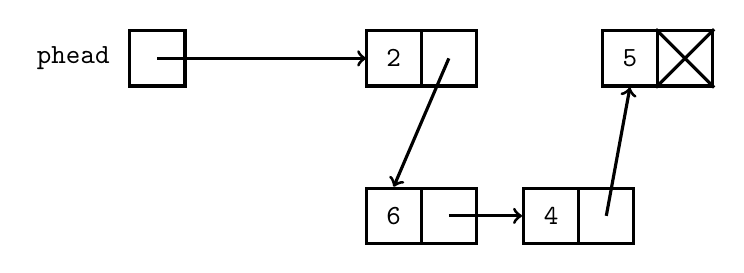
\begin{tikzpicture}

\draw (0.35, 0.35)
  node[draw, line width=0.04cm, , color=black,
       rounded corners=0cm, inner sep=0cm] {

\begin{minipage}[t][0.7cm]{0.7cm}
\mbox{}

\end{minipage}

};\draw (0.35, 0.35) node[color=black] {{\texttt{2}}};
\draw (1.0499999999999998, 0.35)
  node[draw, line width=0.04cm, , color=black,
       rounded corners=0cm, inner sep=0cm] {

\begin{minipage}[t][0.7cm]{0.7cm}
\mbox{}

\end{minipage}

};\draw (1.0499999999999998, 0.35) node[color=black] {{\texttt{}}};
\draw (0.35, -1.65)
  node[draw, line width=0.04cm, , color=black,
       rounded corners=0cm, inner sep=0cm] {

\begin{minipage}[t][0.7cm]{0.7cm}
\mbox{}

\end{minipage}

};\draw (0.35, -1.65) node[color=black] {{\texttt{6}}};
\draw (1.0499999999999998, -1.65)
  node[draw, line width=0.04cm, , color=black,
       rounded corners=0cm, inner sep=0cm] {

\begin{minipage}[t][0.7cm]{0.7cm}
\mbox{}

\end{minipage}

};\draw (1.0499999999999998, -1.65) node[color=black] {{\texttt{}}};
\draw (2.35, -1.65)
  node[draw, line width=0.04cm, , color=black,
       rounded corners=0cm, inner sep=0cm] {

\begin{minipage}[t][0.7cm]{0.7cm}
\mbox{}

\end{minipage}

};\draw (2.35, -1.65) node[color=black] {{\texttt{4}}};
\draw (3.0500000000000003, -1.65)
  node[draw, line width=0.04cm, , color=black,
       rounded corners=0cm, inner sep=0cm] {

\begin{minipage}[t][0.7cm]{0.7cm}
\mbox{}

\end{minipage}

};\draw (3.0500000000000003, -1.65) node[color=black] {{\texttt{}}};
\draw (3.35, 0.35)
  node[draw, line width=0.04cm, , color=black,
       rounded corners=0cm, inner sep=0cm] {

\begin{minipage}[t][0.7cm]{0.7cm}
\mbox{}

\end{minipage}

};\draw (3.35, 0.35) node[color=black] {{\texttt{5}}};
\draw (4.05, 0.35)
  node[draw, line width=0.04cm, , color=black,
       rounded corners=0cm, inner sep=0cm] {

\begin{minipage}[t][0.7cm]{0.7cm}
\mbox{}

\end{minipage}

};\draw (4.05, 0.35) node[color=black] {{\texttt{}}};\draw[line width=0.04cm,black,->] (1.05,0.35) to  (0.35,-1.28);
\draw[line width=0.04cm,black,->] (1.05,-1.65) to  (1.98,-1.65);
\draw[line width=0.04cm,black,->] (3.05,-1.65) to  (3.35,-0.02);
\draw[line width=0.04cm,black] (3.68,0.72) to  (4.42,-0.02);
\draw[line width=0.04cm,black] (4.42,0.72) to  (3.68,-0.02);

\draw (-2.65, 0.35)
  node[draw, line width=0.04cm, , color=black,
       rounded corners=0cm, inner sep=0cm] {

\begin{minipage}[t][0.7cm]{0.7cm}
\mbox{}

\end{minipage}

};\draw (-2.65, 0.35) node[color=black] {{\texttt{}}};\draw[line width=0.04cm,black,->] (-2.65,0.35) to  (0,0.35);

\draw (-3.7199999999999998, 0.35)
  node[draw, line width=0.04cm, , color=white,
       rounded corners=0cm, inner sep=0cm] {

\begin{minipage}[t][0.1cm]{0.1cm}
\mbox{}

\end{minipage}

};\draw (-3.7199999999999998, 0.35) node[color=black] {{\texttt{phead}}};
\end{tikzpicture}

\end{center}


 
\li $T$ is \defone{complete} if it's \lq\lq almost full'' 
except that the last level 
might not have all the nodes. 
Here's a complete binary tree that is not full:

\begin{center}
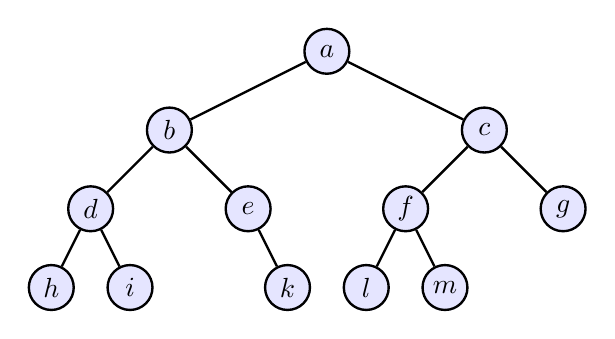
\begin{tikzpicture}

\fill[blue!10] (0.0, 0.0) circle (0.3);
\node [line width=0.03cm,black,minimum size=0.57cm,draw,circle] at (0.0,0.0)(a){};\draw (0.0, 0.0) node[color=black] {$a$};
\fill[blue!10] (-2.0, -1.0) circle (0.3);
\node [line width=0.03cm,black,minimum size=0.57cm,draw,circle] at (-2.0,-1.0)(b){};\draw (-2.0, -1.0) node[color=black] {$b$};
\fill[blue!10] (2.0, -1.0) circle (0.3);
\node [line width=0.03cm,black,minimum size=0.57cm,draw,circle] at (2.0,-1.0)(c){};\draw (2.0, -1.0) node[color=black] {$c$};
\fill[blue!10] (-3.0, -2.0) circle (0.3);
\node [line width=0.03cm,black,minimum size=0.57cm,draw,circle] at (-3.0,-2.0)(d){};\draw (-3.0, -2.0) node[color=black] {$d$};
\fill[blue!10] (-1.0, -2.0) circle (0.3);
\node [line width=0.03cm,black,minimum size=0.57cm,draw,circle] at (-1.0,-2.0)(e){};\draw (-1.0, -2.0) node[color=black] {$e$};
\fill[blue!10] (1.0, -2.0) circle (0.3);
\node [line width=0.03cm,black,minimum size=0.57cm,draw,circle] at (1.0,-2.0)(f){};\draw (1.0, -2.0) node[color=black] {$f$};
\fill[blue!10] (3.0, -2.0) circle (0.3);
\node [line width=0.03cm,black,minimum size=0.57cm,draw,circle] at (3.0,-2.0)(g){};\draw (3.0, -2.0) node[color=black] {$g$};
\fill[blue!10] (-3.5, -3.0) circle (0.3);
\node [line width=0.03cm,black,minimum size=0.57cm,draw,circle] at (-3.5,-3.0)(h){};\draw (-3.5, -3.0) node[color=black] {$h$};
\fill[blue!10] (-2.5, -3.0) circle (0.3);
\node [line width=0.03cm,black,minimum size=0.57cm,draw,circle] at (-2.5,-3.0)(i){};\draw (-2.5, -3.0) node[color=black] {$i$};
\fill[blue!10] (-0.5, -3.0) circle (0.3);
\node [line width=0.03cm,black,minimum size=0.57cm,draw,circle] at (-0.5,-3.0)(k){};\draw (-0.5, -3.0) node[color=black] {$k$};
\fill[blue!10] (0.5, -3.0) circle (0.3);
\node [line width=0.03cm,black,minimum size=0.57cm,draw,circle] at (0.5,-3.0)(l){};\draw (0.5, -3.0) node[color=black] {$l$};
\fill[blue!10] (1.5, -3.0) circle (0.3);
\node [line width=0.03cm,black,minimum size=0.57cm,draw,circle] at (1.5,-3.0)(m){};\draw (1.5, -3.0) node[color=black] {$m$};\draw[line width=0.03cm,black] (a) to  (b);
\draw[line width=0.03cm,black] (a) to  (c);
\draw[line width=0.03cm,black] (b) to  (d);
\draw[line width=0.03cm,black] (b) to  (e);
\draw[line width=0.03cm,black] (c) to  (f);
\draw[line width=0.03cm,black] (c) to  (g);
\draw[line width=0.03cm,black] (d) to  (h);
\draw[line width=0.03cm,black] (d) to  (i);
\draw[line width=0.03cm,black] (e) to  (k);
\draw[line width=0.03cm,black] (f) to  (l);
\draw[line width=0.03cm,black] (f) to  (m);
\end{tikzpicture}

\end{center}


      
\li $T$ is \defone{balanced} if at each node,
every pair of children have heights differ by 0 or 1.
\end{myenum}

\begin{ex}
If $T$ is a balanced tree, does it mean that $T$ is complete?
If $T$ is complete, does it mean that $T$ is balanced?
\qed
\end{ex}

Let $T$ be a $k$--ary tree with height $h$ and the total 
number of nodes is $n$.
At level $\ell$,
there are at most $k^\ell$ nodes.
(Don't forget that the first level that contains only the root
is called level $0$.)
In particular for a binary tree, at level $\ell$, 
there are $2^\ell$ nodes.

Therefore if the height is $h$, $T$ can have at most
\[
k^0 + k^1 + \cdots + k^h = \frac{k^{h+1} - 1}{k-1}
\]
nodes.
(Remember your geometric sum formula?)
In particular, for a binary tree, $T$ can have at most
\[
2^{h+1} - 1
\]
nodes.
Since $T$ has $n$ nodes, we must have the following relation
between $n$ and $h$ for a $k$--ary tree:
\[
h + 1 \leq n \leq \frac{k^{h+1} - 1}{k-1}
\]
And for the case of binary tree, we have
\[
h + 1 \leq n \leq 2^{h+1}
\]

